\documentclass[12pt]{article}
\usepackage{cancel}
\usepackage{graphicx}

\title{Numbers and Counting Course\\
\begin{center}

\includegraphics[width=4em]{ApS_logo.png}
\end{center}
\begin{normalsize}Applied Scholastics, Ferndale \end{normalsize}}
\author{}
\date{}

\begin{document}
\maketitle

\paragraph{Arithmetic and Mathematics}
‘Arithmetic’ is a Greek word meaning ‘methods of counting.’ Arithmetic is all the ways of handling things that can be counted or numbered. It is a starting point for the overall subject of Mathematics which includes arithmetic but is a much broader topic. The word ‘mathematics’ is also from Greek and it meant learning. Usually it is called just 'maths' for short. Maths now means the whole subject that deals with any sort of numbers or shapes, whether or not they have to do with the real world. Any time you are working with things in the real world, meaning things that can be counted or measured, you are using arithmetic.

\begin{enumerate}
\item Write, in your own words, what is arithmetic.
\item Write a sentence that use the word 'arithmetic.'
\item Write, in your own words, what is mathematics.
\item Write a sentence that use the word 'maths.'
\item What is the difference between maths and arithmetic?
\item Write down 5 things that you could do using arithmetic.

\paragraph{Symbol}
A symbol is a thing that has been given a meaning. A symbol stands for or represents something.

\item Write, in your own words, what is a symbol.
\item Write 5 symbols and their meanings.

\paragraph{Number}
A number is an amount of things. It also means the word or symbol used to express the amount of things.

\item Write, in your own words, what is a number.
\item Write 5 sentences using the word 'number.'
\item Write 5 places where you would see numbers.

\paragraph{Numeral}
A numeral is the word or symbol used to express a number. "Four" and "4" are numerals that represent the same number.

\item Write, in your own words, what is a numeral.
\item Write 5 sentences that use the word 'numeral.'
\item What is the difference between a number and a numeral?

\paragraph{Digit}
A digit is a finger. Because people count on their fingers, the numerals in a number are also called digits. A digit is any single symbol that is a numeral in itself or that can stand with other digits as part of a larger numeral. "2" is a digit. "23" is a numeral made up of two digits.

\item Write, in your own words, what is a digit.
\item Write 5 sentences using the word 'digit.'
\item What is the difference between a digit and a number?

\paragraph{Figure}
'Figure' is another word for numeral. That's because a figure is an outline or a drawing of something, and digits and numerals have different shapes and outlines. A person's outline is known as their figure, for example, or diagrams in books are sometimes called figures. 'Figures,' however, usually means numbers, not just numerals. Someone might say "Show me the figures" when working something out. The saying "figure something out" comes from working things out with numbers.

\item Write, in your own words, what are figures.
\item Write 5 sentences using the word 'figure.'

\paragraph{Count}
Count means to note each thing in a group of things to find out how many there are.

\item Write, in your own words, what is counting.
\item Write 5 sentences using the word 'count.'
\item What are 5 things that could be counted?

\paragraph{Numbering} To number things means to give a number to each thing in turn when counting them. Like the chapters of a book are numbered chapter 1, chapter 2, chapter 3, and so on. To number things can also mean to give a group of things the result of a count. You could say that the people of a town number 1000 or that the number of students in the class is 20.

\item Write, in your own words, what it means to number something.
\item Write 5 places where things have been numbered.

\paragraph{Tallies} Tallies are the simplest sort of numbering. For most of our history there were no numbers. There were just marks made as things were being counted. There are different ways of doing that around the world. A tally was originally a stick with notches cut into it. Nowadays the same thing is done but with lines drawn to add each thing to the count. A tally looks like this: $\cancel{||||}\ \cancel{||||}\ \cancel{||||}\ |||.$ Every fifth mark is drawn across the last four marks to make the number easier to see.

\item Write, in your own words, what is a tally.
\item Write 5 sentences using the word 'tally.'
\item Make a tally of the things on your table right now.

\paragraph{Scores}
A score is a scratch mark, and a score is also 20 of something. That comes from making a mark for every 20 of something being counted. Game scores come from keeping a count this way. Also a famous American speech starts with "Four score and seven years ago..." meaning 87 years ago.

\item Write, in your own words, what is a score.
\item Write 5 sentences using the word 'score.'

\paragraph{Roman Numerals} The Roman Empire ruled much of Europe, and large parts of Africa and Asia, for many centuries. They spread their language and their counting system with them. Roman numerals are still used today.\\

Roman numerals use I for 1, V for 5, X for 10, L for 50, C for 100, D for 500, and M for 1000. The V is said to be a shorthand for a spread hand with 5 fingers and the X is said to be two Vs on top of each other.\\

Using these special symbols makes Roman numerals much shorter than tallies.\\

A smaller amount is written either before or after the larger one, indicating that much more or less. That makes them even shorter to write.\\

XVIII in Roman numerals is easier to read and write than $\cancel{||||}\ \cancel{||||}\ \cancel{||||}\ |||$ as a tally.\\

Counting in Roman numerals is I II III IV V VI VII VIII IX X XI XII XIII XIV XV… and so on.\\

Here are the Roman Numerals counting from 1 to 100:\\
\begin{center}
\begin{table}[ht]
\scriptsize
\renewcommand*{\arraystretch}{1.4}
\begin{tabular}{rlrlrlrlrl}
1  & I      & 2  & II      & 3  & III      & 4  & IV     & 5  & V    \\
6  & VI     & 7  & VII     & 8  & VIII     & 9  & IX     & 10 & X    \\
11 & XI     & 12 & XII     & 13 & XIII     & 14 & XIV    & 15 & XV   \\
16 & XVI    & 17 & XVII    & 18 & XVIII    & 19 & XIX    & 20 & XX   \\
21 & XXI    & 22 & XXII    & 23 & XXIII    & 24 & XXIV   & 25 & XXV  \\
26 & XXVI   & 27 & XXVII   & 28 & XXVIII   & 29 & XXIX   & 30 & XXX  \\
31 & XXXI   & 32 & XXXII   & 33 & XXXIII   & 34 & XXXIV  & 35 & XXXV \\
36 & XXXVI  & 37 & XXXVII  & 38 & XXXVIII  & 39 & XXXIX  & 40 & XL   \\
41 & XLI    & 42 & XLII    & 43 & XLIII    & 44 & XLIV   & 45 & XLV  \\
46 & XLVI   & 47 & XLVII   & 48 & XLVIII   & 49 & XLIX   & 50 & L    \\
51 & LI     & 52 & LII     & 53 & LIII     & 54 & LIV    & 55 & LV   \\
56 & LVI    & 57 & LVII    & 58 & LVIII    & 59 & LIX    & 60 & LX   \\
61 & LXI    & 62 & LXII    & 63 & LXIII    & 64 & LXIV   & 65 & LXV  \\
66 & LXVI   & 67 & LXVII   & 68 & LXVIII   & 69 & LXIX   & 70 & LXX  \\
71 & LXXI   & 72 & LXXII   & 73 & LXXIII   & 74 & LXXIV  & 75 & LXXV \\
76 & LXXVI  & 77 & LXXVII  & 78 & LXXVIII  & 79 & LXXIX  & 80 & LXXX \\
81 & LXXXI  & 82 & LXXXII  & 83 & LXXXIII  & 84 & LXXXIV & 85 & LXXXV\\
86 & LXXXVI & 87 & LXXXVII & 88 & LXXXVIII & 89 & LXXXIX & 90 & XC   \\
91 & XCI    & 92 & XCII    & 93 & XCIII    & 94 & XCIV   & 95 & XCV  \\
96 & XCVI   & 97 & XCVII   & 98 & XCVIII   & 99 & XCIX   & 100& C    \\
\end{tabular}
\end{table}
I = 1, V = 5, X = 10, L = 50, C = 100, D = 500, M = 1000\\
\end{center}

\item What does 'Roman' mean?
\item Find Rome on a map.
\item What was the Roman Empire?
\item What are Roman numerals?
\item Are Roman numerals better than tallies? Why?
\item Have you seen Roman numerals before? Where?
\item Write the number of things on your table right now in Roman numerals.
\item Write from 1 to 20 using Roman numerals.

\paragraph{Natural Numbers}
Natural means things that are in the natural world, which is to say the real or physical world. Natural numbers are the numbers that are used for counting things, as in "I have six ducks," or for ordering things, as in "the third duck quacked."

\item What does 'natural' mean?
\item In your own words, what is a natural number?
\item Write 5 examples of natural numbers.

\paragraph{Whole Numbers}
Natural numbers are also called whole numbers, in that they are counting or ordering whole things rather than parts of things. Whole numbers are all numbers greater than zero and, depending on who you talk to, may or may not include zero as a whole number.

\item What does 'whole' mean?
\item In your own words, what are whole numbers?

\paragraph{Cardinal Numbers}
Cardinal means main or the thing that other things depend on. Numbers that are used for counting things are called counting numbers or cardinal numbers.

\item In your own words, what does 'cardinal' mean?
\item In your own words, what are cardinal numbers?
\item In your own words, what are counting numbers?
\item Write 5 examples of cardinal numbers.

\paragraph{Ordinal Numbers}
Numbers that are used for ordering things are called ordinal numbers. Pointing to the "$3{^{rd}}$" duck in a line of ducks uses an ordinal number.

\item In your own words, what does 'order' mean?
\item What does it mean to arrange things in order?
\item In your own words, what does 'ordinal' mean?
\item In your own words, what are ordinal numbers?
\item Write 5 examples of ordinal numbers?

\paragraph{Equals}
Equals means having the same number or amount or size.
The sign for equals, =, is two lines of equal length.

\item What does equals mean, in your own words?

\paragraph{Equations}
An equation means writing that two things are equal each other. Maths problems can be worked out by writing equations. They can be long and complicated, but whenever you use an equals sign you are still writing a simple equation. $2+2=4$ is an equation, for example.

\item What is an equation, in your own words?
\item Write an example of a simple equation.

\paragraph{Arabic Numerals}
The symbols that we use today for numbers, 0123456789, are very old. Them are called Arabic numerals. They first appeared in Europe in the $10^{th}$ century, over 1000 years ago, and they weren't in common use until around the $15^{th}$ century. They came to us though the Arab world though they are originally from India.\\
\begin{center}
{\Huge 0 1 2 3 4 5 6 7 8 9}
\end{center}

\item In your own words, what is 'Arabic'?
\item Make 5 sentences using the word 'Arabic.'
\item In your own words, what is an Arabic numeral?
\item Write out the Arabic numerals.

\paragraph{The Place-Value System}
Until Arabic numerals came to Europe, Roman numerals and systems of tallies and counting stones and so on were used.

The power of these new numbers was in the different way in which they were used.\\

A Roman number only ever stood for that one amount. A Roman V only ever meant five of something, even when it was part of a larger number containing other Roman numerals.\\

The amount that one of these Indian numerals stood for, though, when it was part of a larger number with more than one numeral, changed depending on it’s position in that number. A ‘5’ could mean five of something, or fifty, or five hundred, depending on it’s position.\\

This is called the place-value system. The value of any digit in a number depends on it’s place in that number. The idea is that a digit is read not just as itself but the value of each digit is some multiple more than the digit to it’s right.\\

\paragraph{The Base}
The number that is chosen to multiply each position by is known as as the base. Usually the base is 10, but any number can be used as a base. The base, if it isn't 10, is written as a small number under and to the right of the number. 123 with a base of 8, so each digit is 8 times the value of the digit to its right, is written as $123_8$. It would mean $1 \times 8 \times 8 + 2 \times 8 + 3$. That is 83, which is $(8 \times 10) + 3$ when the same amount is written with a base of 10.

\paragraph{Decimal Base}
We usually use the number 10 as the base, which is why most numbers that you see are called decimal numbers. Decimal means having to do with 10. In decimal numbers, the digit at the right of a number is just itself, but the digit to its left represents 10 times its value, and the next digit to the left is 100 times the value of that digit, and so on.\\

123 is short for $(1 \times 10 \times 10) + (2 \times 10) + (3 \times 1)$.\\

A tally of $\cancel{||||}\ \cancel{||||}\ \cancel{||||}\ \cancel{||||}\ \cancel{||||}\ \cancel{||||}\ \cancel{||||}\ \cancel{||||}\ \cancel{||||}\ \cancel{||||}\ \cancel{||||}\ \cancel{||||}\ \cancel{||||}\ \cancel{||||}\ \cancel{||||}\ \cancel{||||}\ \cancel{||||}\: \cancel{||||}\ \cancel{||||}\ \\ \cancel{||||}\ \cancel{||||}\ \cancel{||||}\ \cancel{||||}\: \cancel{||||}\ |||$ could be written more briefly as CXXIII in Roman numerals, or simply as 123 in Hindu-Arabic numerals.

\item What does 'place-value' mean?
\item What does each of the digits in the number '234' mean?
\item What does 'base' mean in the place-value system?
\item What does 'decimal' mean?
\item Why are the numbers that we mostly use called decimal numbers?
\item How do you show what base you are using when writing a number that isn't a decimal?

\paragraph{Names of Large Numbers}
Large numbers have some special names.

\begin{itemize}
\item A hundred is ten tens, written as 100.
\item A thousand is ten hundreds, 1000.
\item A million is a thousand thousand, 1000,000.
\item A billion is a thousand million, 1000,000,000.\\
(The 'bi-', meaning two, in 'billion' is because a billion once meant a million million.)
\item A trillion is a thousand billion, 1000,000,000,000.\\
(The 'tri-', meaning three, in 'trillion' is because a trillion once meant a million million million.)
\item A googol is 1 followed 100 zeroes, and is where the internet company Google got its name.
\end{itemize}

\paragraph{Commas}
To make decimal numbers easier to read, every third digit is separated by a comma. Thousands, Millions, Billions, and so on can be more easily read off when dealing with larger numbers that way.\\

Is the first digit of 1234567 millions? tens of millions?\\

Written as 1,234,567 it is easier to see that it is millions.\\

Large numbers are read from the left, in groups of three digits.\\

123,456,987,654,321 is read as 123 trillion, 456 billion, 987 million, 654 thousand, 3 hundred and 21.\\

\item How are commas used in writing large decimal number?
\item Write a decimal number with 8 digits, and then put commas every 3 places to make it easier to read.
\item Now read off your large number.

\paragraph{Fractions}
A fraction is a part of a whole number that has been broken into equal-sized parts. They are written as the number of parts and the number of parts that the whole number was broken into. $\frac{3}{4}$ is a fraction where a whole number has been broken into 4 parts and we have 3 of those parts.

\item In your own words, what is a fraction?
\item Write 5 examples of fractions.

\paragraph{Decimal Fractions}
Fractions can also be written as decimal numbers. Just as each digit is ten times the value of the digit to its left, each digit is also a tenth of the value of the digit to its right.

\paragraph{The Decimal Point}
The decimal point is a full stop that marks where the whole number part of a number ends and where the fractional part starts.

Fractions written as decimal numbers are called decimal fractions. They are usually the answers given by calculators, and they are the answers that you get when doing division by hand. Decimal numbers are sometimes just called decimals, and decimal fractions are often just called decimals.

$$12.34 = 10 + 2 + \frac{3}{10} + \frac{4}{100}$$

For a number less than 1, the zero in the units position is still written to make it clear that the number is a fraction. You write 0.25, not just .25.

\item What is a decimal point?
\item In your own words, what are decimal fractions?
\item With a calculator, find $3 \div 4$ and write down what the digits of that answer mean.

\paragraph{Binary Numbers}
Computers use rows of switches that are either off or on to represent the ones and zeroes of numbers with a base of two. This is called binary, where the value of each digit is two times the vale of the digit to it’s left.\\

1101 in binary is $(1 \times 2 \times 2 \times 2) + (1 \times 2 \times 2) + (0 \times 2) + (1 \times 1) = 8 + 4 + 0 + 1 = 13$ in decimal.\\

Doing arithmetic with binary numbers was worked out by mathematician George Boole in the 1800s. Binary numbers are still sometimes called Boolean numbers. The methods that Boole worked out for binary numbers are wired into all modern computers. The computer's work is all done in binary and then converted into decimal for human readers.

\item What does binary mean?
\item What does each position in a binary number mean?
\item What is the binary number $1101_2$ when written as a decimal number?

\paragraph{Octal}
Octal numbers, base 8, are also sometimes used with computers because each octal digit is equivalent to a group of three binary digits, which makes the electronics required simpler in running LED displays that are made up of 7 LEDs.\\

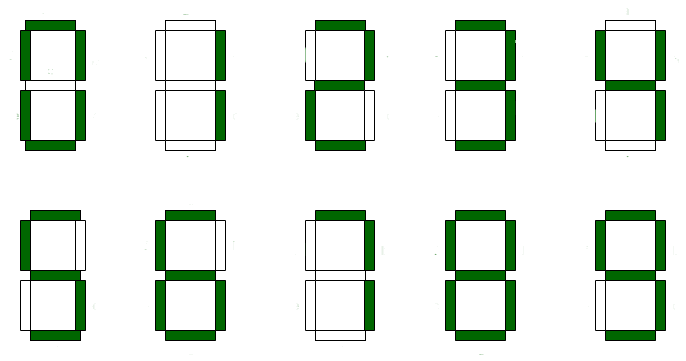
\includegraphics[width=0.5\textwidth]{7segment}

1101 binary (13 decimal) (or, placed into groups of 3 binary digits, 001 101) is 15 in octal (1 x 8 + 5 x 1.) Notice that 001 binary is 1 octal and 101 binary is 5 octal - the binary values that are seen in the octal digits.\\

\item What does octal mean?
\item What does each position in an octal number mean?
\item What is the octal number $123_8$ when written as a decimal number?

\paragraph{Hexadecimal}
You can also come across a base of sixteen used with computers, called hexadecimal, which uses the numbers 0 to 9 and then the letters A to F for 16 digits.\\

AF23 in hexadecimal means	(A x 4096) + (F x 256) + (2 x 16) + 3
= (10 x 4096) + (16 x 256) + (2 x 16) + 3
= 40960 + 4096 + 32 + 3
= 45091 in decimal.\\

Hexadecimal is used for work with computers because each digit of a hexadecimal number is a four digit binary number.\\

For example, 1011 binary (11 decimal) is simply B in hexadecimal. Binary numbers in computers are typically 64 digits long so writing them in hexadecimal for human readers makes them much shorter and easier to deal with.\\

\item What does hexadecimal mean?
\item What does each position in a hexadecimal  number mean?
\item What is the hexadecimal number $1C2_16$ when written as a decimal number?

\paragraph{Vigesimal}

You may remember that a score is a scratch mark, and that a score is also 20 of something, and that that comes from making a mark for every 20 of something being counted. That is known as the vigesimal system. Vigesimal means based on twenties. It can still be found, for example, in the way that the French count things. 20 is used as a base so that 70 is said as sixty-ten (soixante-dix, in French), and 80 is said as four twenties (quatre-vingts.)

\item What does vigesimal mean?
\item Write a sentence using the word 'vigesimal.'

\begin{center}
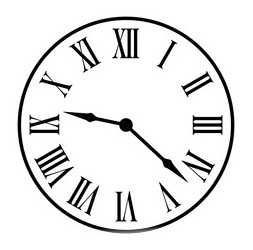
\includegraphics[width=0.5\textwidth]{old-fashion-vintage-clock-face}
\end{center}

\paragraph{Sexagesimal}
The other number system that is commonly used around the world uses 60 as a base and is called the sexagesimal system. Sexigesimal means based on 60s. 60 is a very handy number to use because it divides evenly into so many other numbers – 30, 15, 20, 10, 5, 4, 3, and 2. It was first used by astronomers about three thousand years ago and it is why, among other things, there are 24 hours in a day, 60 minutes to an hour, sixty seconds to a minute, and 360 degrees in a circle.

\item What does sexagesimal mean?
\item What are some things that are based on the sexagesimal system?

\end{enumerate}
\end{document}
